\section{Course Overview}

ME 570: Control of Mechanical Systems is a mixed class with two lectures and one lab every week. The lectures focus on teaching
the principles and theory of controls while the lab focuses on designing and testing control systems. Most labs are dedicated to
using and designing PID controllers using different methods, such as frequency analysis or pole analysis.

To complete the labs, the class makes use of a custom motor rig called the motorlab. To go along with the motorlab, a graphical 
user interface for controlling the motorlab was also created by Dale Schinstock. This GUI runs as an application through MATLAB 
and allows the students to both send commands to the motor and collect runtime data from the motor.

Controls also relies heavily on MATLAB for the completion of lab and homework assignments. All work is done using .mlx files through a 
licensed copy of MATLAB for a more interactive working environment. To access the controls related commands, a package called 
the Controls Toolbox has to be purchased from MATLAB. 

While Controls uses programming more than any class besides ME 400, little to no instruction is provided on how to program in MATLAB.
The first lab is dedicated to taking the MATLAB Onramp starter course, which takes about 1 to 2 hours to complete. However, the 
Onramp does not address most of the work done in Controls, such as plotting and transfer functions. The Onramp does teach students
the basics of MATLAB syntax, but most students come out of the Onramp just as confused by MATLAB as they were going in.

This disconnect between students and MATLAB becomes a barrier that prevents students from understanding controls. Many students
spend more time trying to understand MATLAB than they do learning controls. 

\section{Lab Assignment Redesigns}

Since ME 570 already fully utilizes programming in the course, no new assignments are being created. Instead, three pre-existing
labs have been translated from MATLAB to Python. While MATLAB is the industry standard when it comes to control systems, the
license is expensive, students do not have a solid understanding of it, and we do not make use of its most powerful feature,
Simulink. In addition to this, Python has a library, aptly named "control," which has a MATLAB module that imitates the Control
Toolbox, both in form and functionality, from MATLAB. In combination with Jupyter Notebooks and a few custom plotting modifications,
using Python will give a very similar experience to MATLAB, and will give students that pursue the field of controls any easy
transition to MATLAB. 

All three translated labs make use of the motorlab, which has had its GUI turned into an application, courtesy of the MATLAB
Compiler. This allows the application to be run from an app icon or from the terminal. These labs also make use of a custom plot
command. The plot command hijacks the standard matplotlib plot command and adds the ability to create data tips. The
direction of the data tip changes based on which mouse click is used, and a double click in the plot window will remove all data tips.
More custom functions could be added later to imitate MATLAB functionality as needed, but this was the only one required for
completing these labs.

The first translated lab, Lab 4, is a standard controls assignment that makes use of the motorlab, reading the csv output from the
motorlab, and plotting the results. 

\assignments{ME 570: Assignment 1}
\label{control_assignment_1}

\begin{tcolorbox}[breakable, enhanced jigsaw, title=ME 570: Assignment \ref{control_assignment_1}, 
    colframe=ksu-purple, colback=ksu-gray]

    \textbf{Problem Statement}
    \parindent15pt

    For the full problem statement, please see Appendix \ref{appendix:appendix_github}. Estimate
    the damping ratio by fitting an envelope to the step response.
    
    \tcblower
    \textbf{Problem Solution}
    \parindent15pt

    For the full solution, see Appendix \ref{appendix:appendix_github}. The solution shown below
    highlights the use of data from the motorlabGUI and plotting with custom data tips.

    To achieve an environment similar to MATLAB, the following imports are required at the top of the file.

\begin{python}
%matplotlib widget
from matplotlib.pyplot import figure, xlabel, ylabel, legend, show, title, xlim, ylim
from custom_functions import plot
from control.matlab import tf, step
from numpy import polyfit, array
from math import pi, sqrt
from pandas import read_csv
\end{python}

\begin{python}
J = 1.1e-5 + 0.19e-5
ks = k_estimate
Kdc = kt/ks
wn = sqrt(ks / J)
zeta_estimate = 0.05
 
# Generate a step response from a first order system 
# with a pole equal to the real part of the
# 2nd order poles
real_part = zeta_estimate * wn
envelope_TF = tf(Kdc * real_part, [1, real_part])
[envelope_y, envelope_time] = step(envelope_TF)
\end{python}

The following code assumes that the motorlabGUI data was collected
and saved with the name ``stepdata.csv.'' Here, `read\_csv' and
`iloc' from the `pandas' library are used for clean file reading.

\begin{python}
# Extract data from the generated step response
stepdata = read_csv("stepdata.csv", header=None)

# extract time column of the data matrix
dataTime = stepdata.iloc[:,0]

# extract third angle column of the data matrix
dataAngle = stepdata.iloc[:,2]

# convert to rad
dataTh = kdr * dataAngle
\end{python}

After the data has been loaded into the workbook, a graph of the step
response can be plotted.

\begin{python}
plot(dataTime, dataTh, envelope_time, envelope_y, '--')
ylabel('Angular Position (rad)')
xlabel('Time (sec)')
ylim(-0.01, 0.55)
xlim(-0.01, 0.7)
title('Step Response Data with Estimated Envelope')
legend(['step response from Motorlab','estimated envelope'])
show()
\end{python}

\begin{center}
    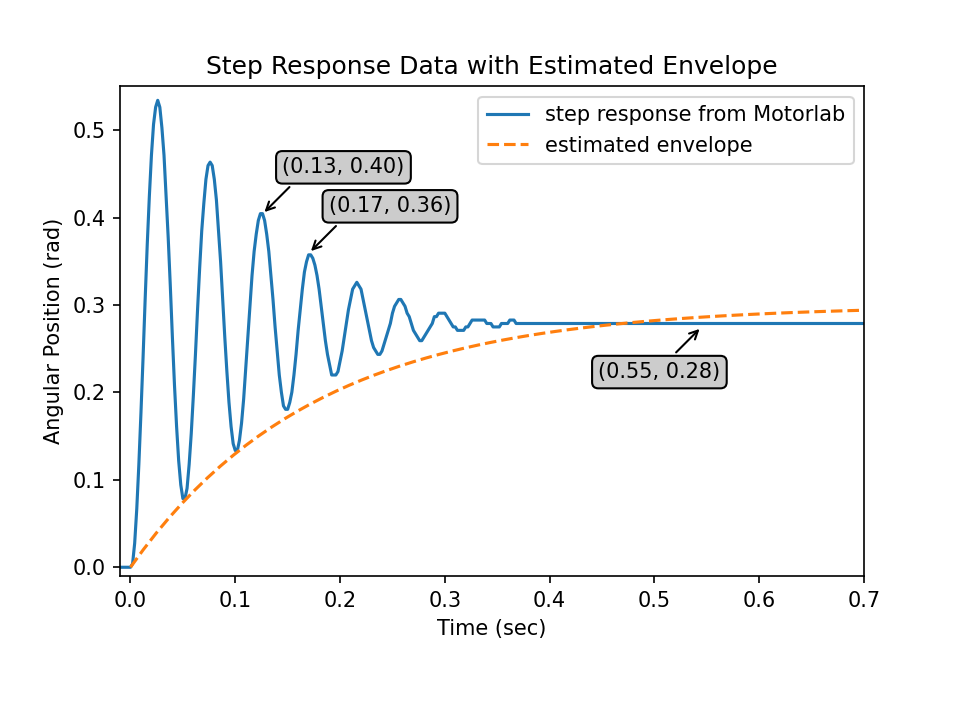
\includegraphics[width=\textwidth]{controls-assignment1-graph.png}
\end{center}

\end{tcolorbox}

The second lab, Lab 10, builds on Lab 4 by adding root locus plots and sisotool. While the
sisotool command in Python is not as powerful as the full designer in MATLAB, it does allow 
for interactive plots where moving poles updates the graphs automatically. 

\assignments{ME 570: Assignment 2}
\label{control_assignment_2}

\begin{tcolorbox}[breakable, enhanced jigsaw, title=ME 570: Assignment \ref{control_assignment_2}, 
    colframe=ksu-purple, colback=ksu-gray]

    \textbf{Problem Statement}
    \parindent15pt

    For the full problem statement, please see Appendix \ref{appendix:appendix_github}. Create a
    controller for the motorlab and plot the poles using sisotool.
    
    \tcblower
    \textbf{Problem Solution}
    \parindent15pt

    For the full solution, see Appendix \ref{appendix:appendix_github}. Below is an example of 
    setting up a transfer function and a controller and then using sisotool to analyze the system.

\begin{python}
b = 3e-5
kdr = 180/pi
J = 1.29e-5
kt = 0.05

s = tf('s')
Gm= kt*kdr / (J*s**2+b*s)
Gc2 = 10*.00007 + .00007*s
\end{python}

After the transfer function and controller have been made, sisotool can be used to adjust the poles.

\begin{python}
figure()
sisotool(Gc2*Gm)
show()
\end{python}

Grabbing and moving the black squares will allow the user to move the pole locations.

\begin{center}
    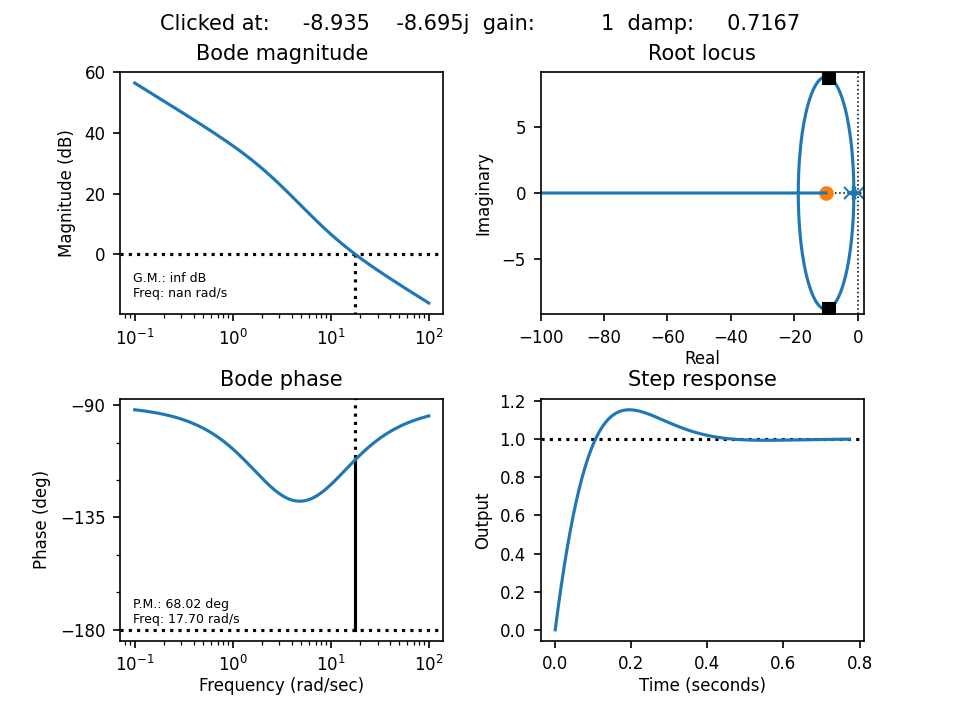
\includegraphics[width=\textwidth]{controls-assignment2-sisotool.png}
\end{center}
\end{tcolorbox}

The third lab, Lab 13, focuses on frequency response design methods and utilizes Bode plots.

\assignments{ME 570: Assignment 3}
\label{control_assignment_3}

\begin{tcolorbox}[breakable, enhanced jigsaw, title=ME 570: Assignment \ref{control_assignment_3}, 
    colframe=ksu-purple, colback=ksu-gray]

    \textbf{Problem Statement}
    \parindent15pt

    For the full problem statement, please see Appendix \ref{appendix:appendix_github}. Given the 
    natural frequency and dc gain derived from the table (not shown here), construct a new transfer 
    function, that will hopefully better match the data.
    
    \tcblower
    \textbf{Problem Solution}
    \parindent15pt

    For the full solution, see Appendix \ref{appendix:appendix_github}. The followign code is an
    example of using Bode in Python to do frequency analysis.

\begin{python}
wn = 19.18*2*pi # natural freq from data (rad/s)
Kdc = 23 # dc gain from data in deg/Amp
Mwn = 540 # magnitude ratio at wn from data in deg/Amp
zeta = Kdc/Mwn/2 # calc damp ratio using Mwn and Kdc
Gnew = (Kdc*wn**2) / (s**2 + 2*zeta*wn*s + wn**2)

mnew, pnew, wnew = bode(Gnew) # get mag, phase, freq
mnew = 20 * log10(mnew)
pnew = (180 / pi) * pnew # Convert radians to degrees
\end{python}

With the new data models complete, graph them using a logarithmic plot.

\begin{python}
figure()
subplot(2, 1, 1)
semilogx(wnew, mnew, w, m, wdata, magdata, '*')
title('Bode Plot')
ylabel('magnitude (dB)')
xlabel('freq (rad/s)')

subplot(2, 1, 2); 
semilogx(wnew, pnew, w, p, wdata, phdata, '*')
ylabel('phase (deg)');
xlabel('freq (rad/s)')
legend(['improved', 'original', 'data'])
show()
\end{python}

\begin{center}
    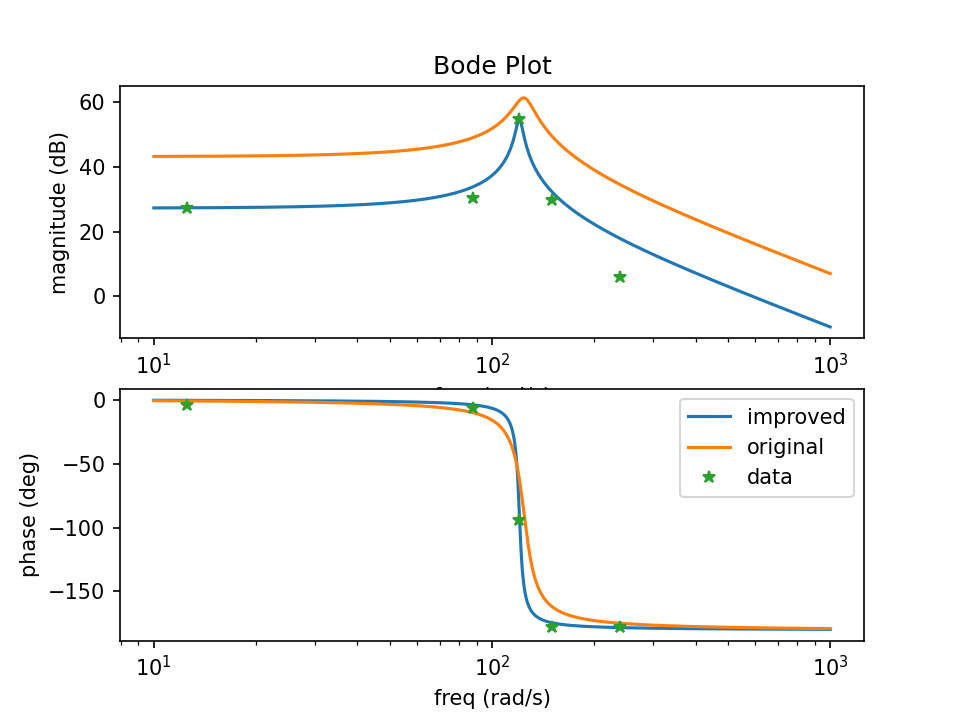
\includegraphics[width=\textwidth]{controls-assignment3-bode.png}
\end{center}
\end{tcolorbox}

The labs chosen aim to showcase how the major features used in MATLAB can be emulated in Python. Some features, like Simulink, have
no direct correlation. However, Simulink is only used in one lab, and students only need to make two small changes. Python also
requires more library imports, but these can all be handled by the skeleton and do not pose much concern.

Since no new assignments are being added to the class, the learning objectives for the class do not change.

\section{Project Deliverables}

In the GitHub repository associated with this paper, which can be found in Appendix \ref{appendix:appendix_github},
the folder titled ``9-control-of-mechanical-systems'' contains the lab assignments, code skeletons, and solutions for the three
lab assignments explained above. The folder also contains a README that details what is in each file and what software is needed 
to complete the assignments. 

The act of integrating these labs into the class would not be as simple as the integrations for other classes. Since every lab 
uses MATLAB, the other 11 labs would also need to be translated. In addition to this, every computer in the lab would need to 
get the correct applications, extensions, and motorlabGUI executable installed. Instructions for installing everything needed 
can be found in the ``usage-and-installation'' folder in the GitHub repository.
